\documentclass[num-refs]{wiley-networks}

\usepackage{float}

\papertype{Paper}
\paperfield{Quantum software development}

\title{Quantum error correction on the quantum Fourier transform algorithm}

\author[1\authfn{1}]{Benjamin Eder}

\corremail{beder@hm.edu}

\fundinginfo{Munich University of Applied Sciences}

\runningauthor{Benjamin Eder}


\begin{document}

    \maketitle

    \begin{abstract}
        Lorem ipsum dolor sit amet, consetetur sadipscing elitr, sed diam nonumy eirmod tempor invidunt ut labore et dolore magna aliquyam erat, sed diam voluptua. At vero eos et accusam et justo duo dolores et ea rebum. Stet clita kasd gubergren, no sea takimata sanctus est Lorem ipsum dolor sit amet. Lorem ipsum dolor sit amet, consetetur sadipscing elitr, sed diam nonumy eirmod tempor invidunt ut labore et dolore magna aliquyam erat, sed diam voluptua. At vero eos et accusam et justo duo dolores et ea rebum. Stet clita kasd gubergren, no sea takimata sanctus est Lorem ipsum dolor sit amet.
    \end{abstract}

%    \hrule

    \tableofcontents

    \setlength{\parskip}{0.2cm}%

    \section{Introduction}
\label{sec:introduction}

While quantum computing is still at an early stage, many quantum algorithms seem to provide drastic accelerations compared to their current classical counterparts.
One of the best known of these is Shor's algorithm which is almost exponentially faster than the currently most efficient factoring algorithms and thus poses a threat to cryptosystems that rely on the factoring problem being hard to solve~\cite{Shor}.

However building a quantum computer and making use of it is not an easy task.
It is essential for such a quantum system to be isolated from unknown interactions with the external world which may mess up the internal state and thus the received results~\cite[p. 34]{Milburn}.
Simultaneously those systems need to be manipulable to an extent in order to be able to implement quantum gates or encoding starting states for the individual qubits~\cite{Matuschak2019}.

Qubits on their own, as well as in an entangled state are error prone in the presence of \emph{noise} and \emph{decoherence}~\cite[p. 34]{Milburn}.
Both appear even with current quantum systems.
To protect fragile quantum information and build fault-tolerant quantum computers, we use quantum error correction (\emph{QEC})~\cite[p. 46998]{Li}.
QEC is achieved by using special codes to encode quantum information~\cite[p. 113]{deBrito}.
Most codes are based on redundancy, which means the introduction of multiple qubits, instead of just one, that carry the information~\cite[p. 113]{deBrito}.

\subsection{Background}
\label{subsec:background}

This examination paper was written in the context of the lecture \emph{Quantum Software Development}, which was held by \emph{Prof. Dr. Sabine Tornow} in the summer semester of 2020 at the \emph{Munich University of Applied Sciences}.

\subsection{Description}

\citeA[p. 46998]{Li} mentions that quantum error correction is already achievable on platforms such as \emph{IBM Q Experience}~\cite{IBMQExperience}.
Using that platform this paper describes an attempt to correct bit-flip errors in a quantum circuit performing a quantum Fourier transform on a real quantum device.
Before testing on the actual computer provided by the Cloud service, the needed circuit has to be modelled and tested using a Simulator.
IBM provides a library \texttt{Qiskit} which is usable with the programming language \texttt{Python} and offers the needed Simulator as well as an interface to use the IBM Q Experience platform~\cite{Qiskit}.

\subsection{Structure}
\label{subsec:structure}

To give an overview over the structure of the paper, the following sections are quickly described.

The paper starts with a quick recapitulation about the \textbf{basic concepts}, namely \emph{quantum error correction}, \emph{quantum Fourier transform} and \textbf{related work}.
Afterwards the \textbf{used methods and tools} are introduced with which the quantum circuit is modelled and tested, followed by the actual \textbf{implementation}.
The resulting circuit is then tested and results from the simulator as well as the real quantum computer \textbf{analyzed}.

A \textbf{conclusion} about the resulting paper is drawn at the end with some \emph{proposals for further studies}.

    \section{Basic concepts}
\label{sec:basic-concepts}

Before delving into the details of implementing the quantum circuit with error correction, a brief recapitulation about the basic concepts is helpful.
To keep it short, only the \emph{immediately needed} concepts are described.
It is assumed that the reader is already familiar with the principles of quantum computing.

\subsection{Quantum Error Correction}
\label{subsec:qec}

Error correction to fight noise has been around in the classical computing domain for a long time~\cite[p. 459]{benenti2004principles}.
It has been discovered that one of the key ingredients is \textbf{redundancy}~\cite[p. 459]{benenti2004principles}.
Fortunately the same happens to be true for the quantum domain~\cite[p. 46998]{Li}.
To apply a simple error correction one could use three instead of just one qubit carrying the same information just like in classical computing.
Unfortunately when dealing with qubits we have to obey some additional rules.

\begin{enumerate}
    \item There is the no-cloning theorem which means it is impossible to just copy quantum states~\cite[p. 460]{benenti2004principles}.
    We are left with encoding the same starting states of individual qubits or using \texttt{CNOT} gates to mimic copying behavior~\cite[p. 461]{benenti2004principles}.
    The approach using \texttt{CNOT} gates is shown in figure~\ref{fig:cnot-circuit}.
    \begin{figure}[H]
        \centering
        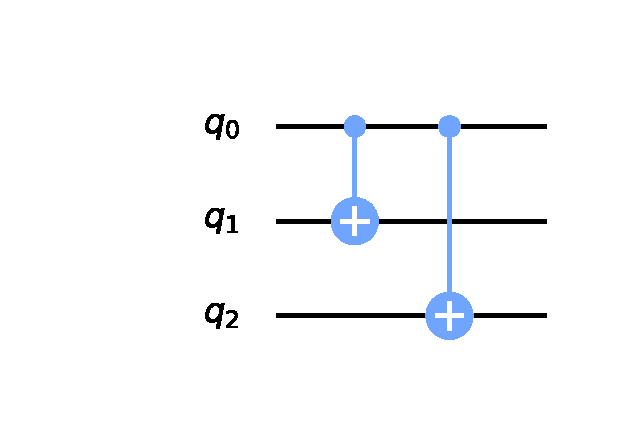
\includegraphics[width=0.5\textwidth]{res/cnot_circuit.pdf}
        \caption{\texttt{CNOT} gates used to encode the information of qubit \(q_0\) onto three.}
        \label{fig:cnot-circuit}
    \end{figure}
    \item Measuring a qubit causes its state to collapse~\cite[p. 460]{benenti2004principles}.
    Thus, we cannot just measure the state and correct it as it will destroy any superposition we ideally want to continue working with.
    The introduction of ancillary qubits that measure the \emph{error syndrome} solves that problem~\cite[p. 463]{benenti2004principles} as shown in figure~\ref{fig:reading-ancilla-qubits-circuit}.
    \begin{figure}[H]
        \centering
        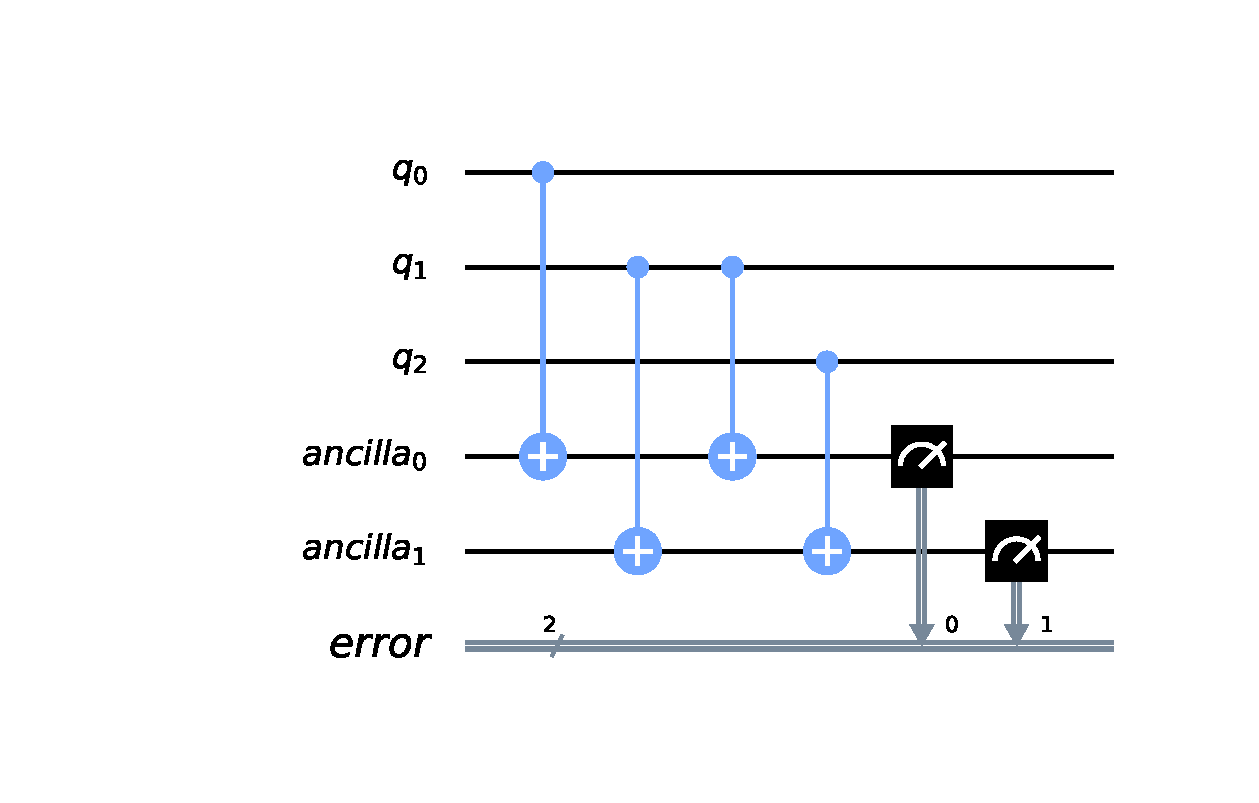
\includegraphics[width=\textwidth]{res/reading_ancilla_qubits_circuit.pdf}
        \caption{Measuring the \emph{error syndrome} using ancillary qubits.}
        \label{fig:reading-ancilla-qubits-circuit}
    \end{figure}
    The ancillary qubits under utilization of \texttt{CNOT} gates allow the comparison of the quantum information that is present in the redundant qubits.
    Thus, the following table shows the possible outcomes of the error syndrome which shows whether there was an error and even where it happened.
    \begin{center}
        \begin{tabular}{ r c l }
            \texttt{00} & \(\Rightarrow\) & No error happened \\
            \texttt{01} & \(\Rightarrow\) & Error happened in \(q_0\) \\
            \texttt{10} & \(\Rightarrow\) & Error happened in \(q_2\) \\
            \texttt{11} & \(\Rightarrow\) & Error happened in \(q_1\)
        \end{tabular}
    \end{center}
    Based on the results we are able to correct the errors.
    \item Compared to classical computing where only a bit-flip error is possible, qubits are additionally prone to phase-flips and even worse to a number of those errors.
    In the process of a quantum computation noise may apply multiple small rotations on the state~\cite[p. 460]{benenti2004principles}.
    \citeA[p. 465]{benenti2004principles} show that the same method for correcting bit-flips can be used to detect phase-flips when we transform from the \(\{|0\rangle, |1\rangle\}\) computational basis to \(\{|+\rangle, |-\rangle\}\) as a bit-flip becomes a phase-flip and vice versa.
\end{enumerate}

Since in this paper we will attempt to correct bit-flip errors, there is nothing more than this to understand how it works.

\subsection{Quantum Fourier Transform}
\label{subsec:quantum-fourier-transform}

In the course of this paper we try to correct errors in a quantum Fourier transformation (\emph{QFT}) algorithm.
Therefore, it is certainly advantageous to repeat the underlying concepts.

The QFT maps a quantum state \(|\psi\rangle\) on another quantum state \(|\alpha\rangle\) with the following definition~\cite[p. 1]{Weinstein_2001}.

\[
    QFT_M|\psi\rangle \rightarrow \frac{1}{\sqrt{M}} \sum_{k=0}^{M-1} e^{2 \pi i a k/M} |\alpha\rangle
\]

This can be expressed as a unitary matrix which can be decomposed into several quantum gates~\cite[p. 2]{Weinstein_2001}.
For example the one-qubit QFT is just the Hadamard gate~\cite{QiskitTBQFT}.

\[
    H = \frac{1}{\sqrt{2}}
    \begin{bmatrix}
        1 & 1 \\
        1 & -1
    \end{bmatrix}
\]

Another example is the two-qubit \(QFT_4\) taken from~\citeA[p. 2]{Weinstein_2001}.

\[
    QFT_4 = \frac{1}{2}
    \begin{bmatrix}
        1 & 1 & 1 & 1 \\
        1 & i & -1 & -i \\
        1 & -1 & 1 & -1 \\
        1 & -i & -1 & i
    \end{bmatrix}
\]

That matrix can be decomposed into the circuit shown in figure~\ref{fig:qft4-circuit}~\cite{QiskitTBQFT}.

\begin{figure}[H]
    \centering
    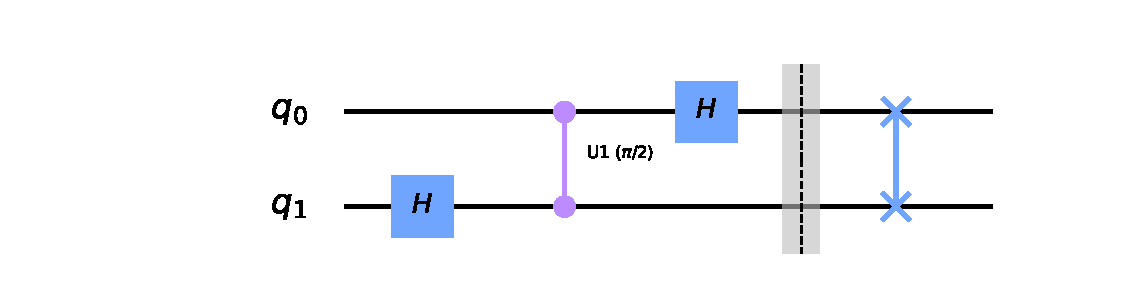
\includegraphics[width=0.7\textwidth]{res/qft4_circuit.pdf}
    \caption{Circuit for the two-qubit QFT \(QFT_4\).}
    \label{fig:qft4-circuit}
\end{figure}

\clearpage

All those matrices and circuits follow the same pattern~\cite{Yin2020Jun}:

\[
    QFT_M =
    \frac{1}{\sqrt{M}}
    \begin{bmatrix}
        1 & 1 & 1 & 1 & \ldots & 1 \\
        1 & \omega & \omega^2 & \omega^3 & \ldots & \omega^{M-1} \\
        1 & \omega^2 & \omega^4 & \omega^6 & \ldots & \omega^{2M-2} \\
        1 & \omega^3 & \omega^6 & \omega^9 & \ldots & \omega^{3M-3} \\
        \ldots & \ldots & \ldots & \ldots & \ldots & \ldots \\
        1 & \omega^{M-1} & \omega^{2M-2} & \omega^{3M-3} & \ldots & \omega^{(M-1)(M-1)} \\
    \end{bmatrix}
\]

where \(\omega = e^{\frac{2\pi i}{M}}\).
Even a matrix of any size can be broken down into a circuit as shown in Figure~\ref{fig:qft-generic-circuit}.
Note that the shown controlled \texttt{R} gate is really just a rotation around the Z-axis with angle \(\frac{\pi}{2^{k-1}}\).

\begin{figure}[H]
    \centering
    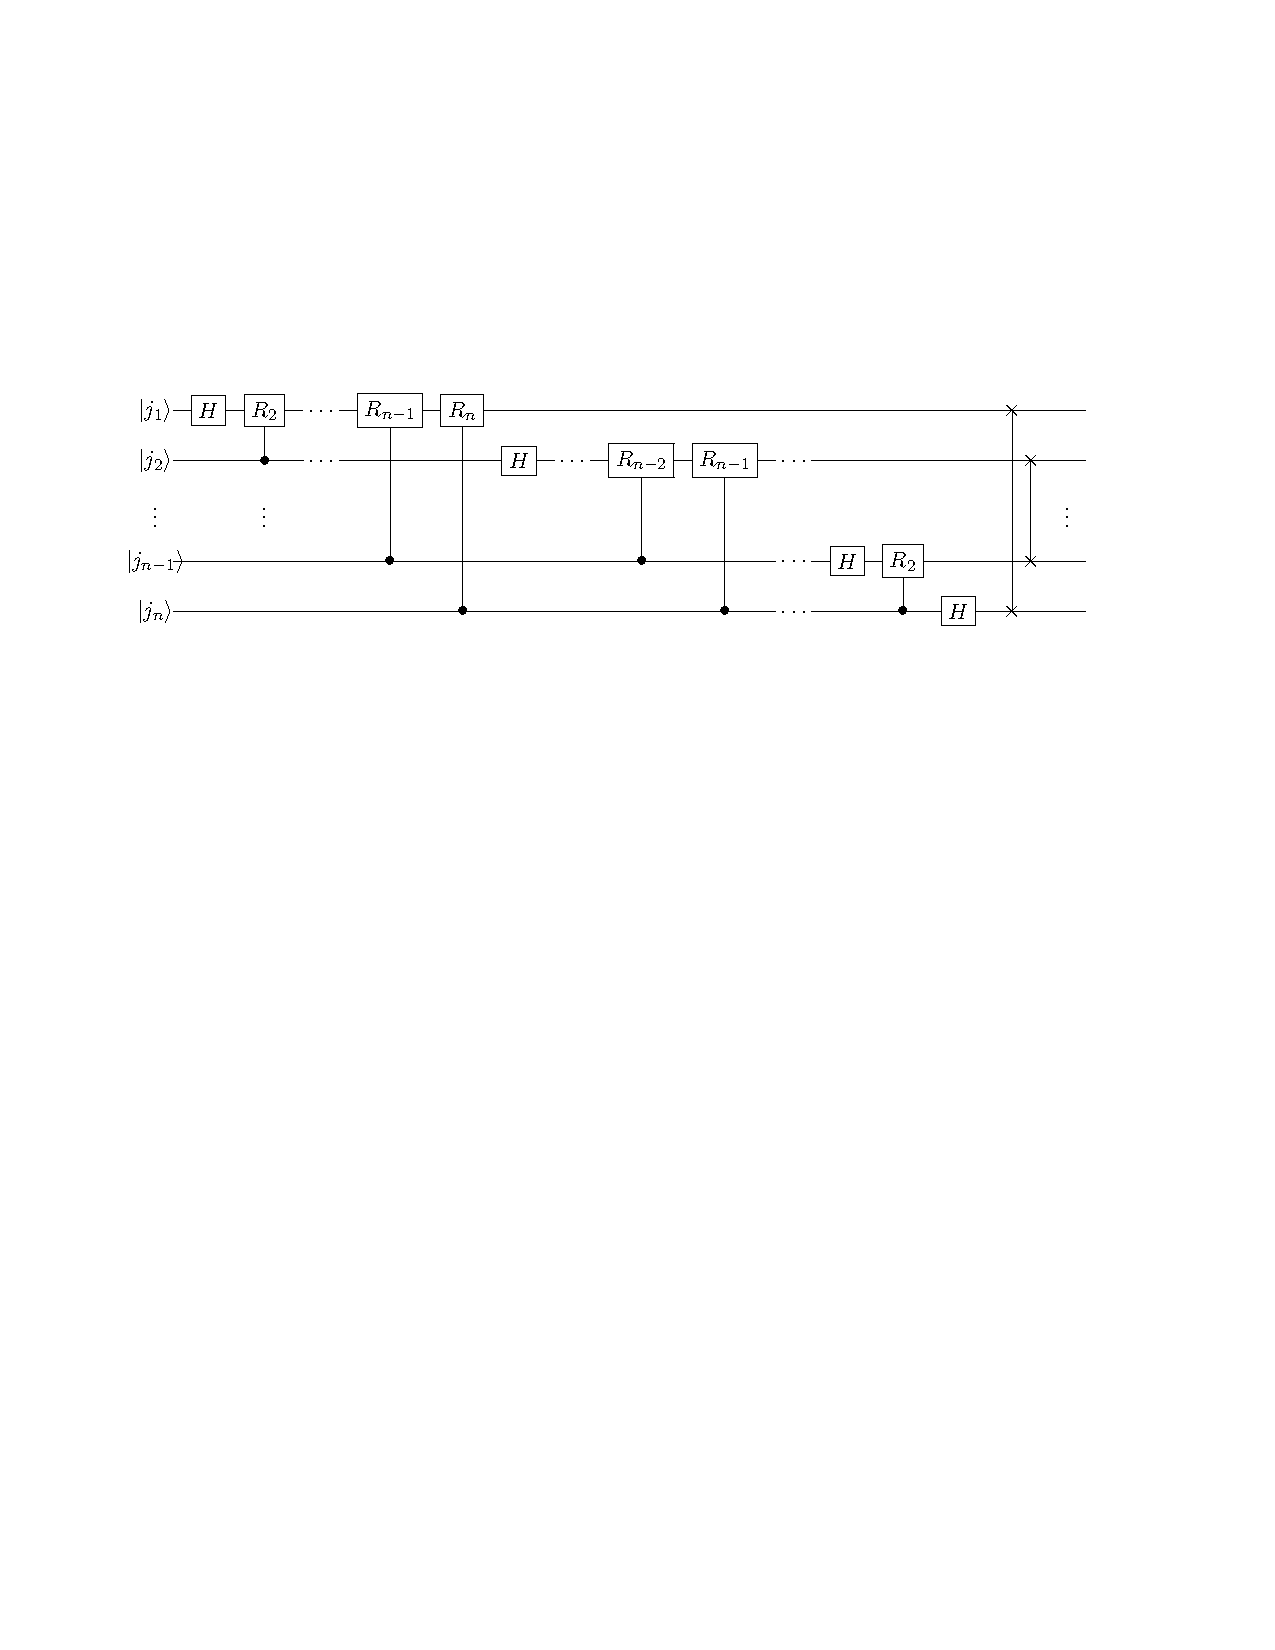
\includegraphics[width=\textwidth]{res/qftm_circuit.pdf}
    \caption{\(QFT_M\) circuit taken from \protect\citeA{VANJURGEN}}
    \label{fig:qft-generic-circuit}
\end{figure}

Now we have enough information at hand to realize such a circuit with the tools and methods introduced and used in the following sections.

    \section{Related work}
\label{sec:related-work}

In the last section some basic concepts about quantum error correction were introduced.
For this paper we do not need more.
But there is certainly more about that comparatively new topic in the quantum domain.
This section will provide an overview of past and current developments in QEC.

It all began the last 90s where the noise has been discretized into discrete error models, namely bit- and phase-flip errors~\cite[p. 46999]{Li}.
Shor has developed a quantum error correction code (QECC) that successfully applies the previously reviewed bit-flip and phase-flip error circuits to protect against any type of error with 9 qubits~\cite[p. 46999]{Li}.
That event was followed by Calderbank, Shor and Steane each constructing the so-called CSS codes which were adopted from the theory of classical linear codes~\cite[Chapter: Quantum Error Correction, p. 24]{Preskill}.
It was discovered that the minimum amount of qubits needed to protect a single qubits information against any error is five~\cite[p. 46999]{Li}.

Since there seems to be no improvement to protect against any error, scientists moved on to protect against specific errors instead, thereby reducing the amount of qubits even further~\cite[p. 46999]{Li}.
That is especially useful when the error-source is known and thus can be excluded.

Discrete error models are not like the real world and rely on idealized scenarios.
For example they simplify that errors occur on qubits independently, thus there is currently increasing effort in implementing continuous error models.~\cite[p. 46999]{Li}.

    \section{Methods and tools}
\label{sec:methods-and-tools}

As a reminder, we will try to correct bit-flip errors of a quantum Fourier transform circuit.
Therefore, some tools and methods are selected and presented in this section.

\subsection{Qiskit}
\label{subsec:qiskit}

Since we are already familiar with the quantum computing software development framework \texttt{Qiskit}, it is an obvious choice.
Its tight coupling with IBM Quantum Experience and thus accessible quantum devices allow testing quantum circuits in a real environment~\cite{IBMQAccount}.
Besides that the framework offers a simulator capable of testing the created code as well as adding a noise model to imitate real quantum computer behavior, which we want to fight using our quantum error correction solution~\cite{QiskitNoiseModel}.

\subsection{Python}
\label{subsec:python}

Qiskit is a library for the programming language Python.
Thus we have to use it.
Additionally, Pythons popularity soared in the last years especially in scientific areas, making it one of the most popular programming languages~\cite{StackOverFlowDevSurveyTechnolgies}.
Thus, most people reading this paper should easily be capable of understanding the included code snippets, improving accessibility.

The precise version of the language is \texttt{Python 3.8.2} which is used throughout this paper.
There is no other reason for choosing that exact version other than \texttt{Qiskit} is supporting it and it is an up-to-date version of the language at the time of writing.

\subsection{JupyterLab}
\label{subsec:jupyter-lab}

\texttt{JupyterLab} is a web-based user interface for Project Jupyter~\cite{JupyterLabDocs}.
It is an open-source project to support interactive data science and scientific computing~\cite{ProjectJupyter}
One of its components called \emph{Jupyter Notebooks} will be used to quickly write and test Python code with additional support for LaTeX and Markdown to document that code more clearly~\cite{JupyterLabOverview}.

In addition, the code is also included in the annex to this document in order to ease the reproduction of the work of this paper.

    \section{Implementation of a QECC}
\label{sec:implementation}

In this section we are finally using the tools and methods presented in the last section to apply the quantum error correction (bit-flips) for the quantum Fourier transform.

\subsection{Implementing the quantum Fourier transform circuit}
\label{subsec:implementing-quantum-fourier-transform-circuit}

First and foremost it would make certainly sense to build the proposed QFT circuit and see if it actually works on a simulator and a real quantum device.
Recalling the basic concepts chapter we have already seen a generic circuit in figure~\ref{fig:qft-generic-circuit} that can be rebuilt using Qiskit.
The controlled \texttt{R}-gate is a rotation around the Z-axis which can be realized in \texttt{Qiskit} using a controlled \texttt{U1} gate~\cite{ControlledU1Gate}.

Before using \emph{Qiskit} and building the circuit we need to set up the code by listing the needed imports in appendix~\ref{subsec:qft-circuit-qiskit-necessary-imports} for \emph{Python}.
Afterwards we can follow the circuit in figure~\ref{fig:qft-generic-circuit} and implement it iteratively for any size in Qiskit as seen in appendix~\ref{subsec:qft-function}.
That allows us creating an arbitrarily big circuit.
One example circuit graph for 4 input qubits is created and shown in figure~\ref{fig:qft-4-qubit-circuit}.
Note that the circuit is mirrored vertically compared to the reference circuit, as Qiskit is ordering the qubits differently compared to most resources~\cite{QiskitGettingStarted}.

\begin{figure}[H]
    \centering
    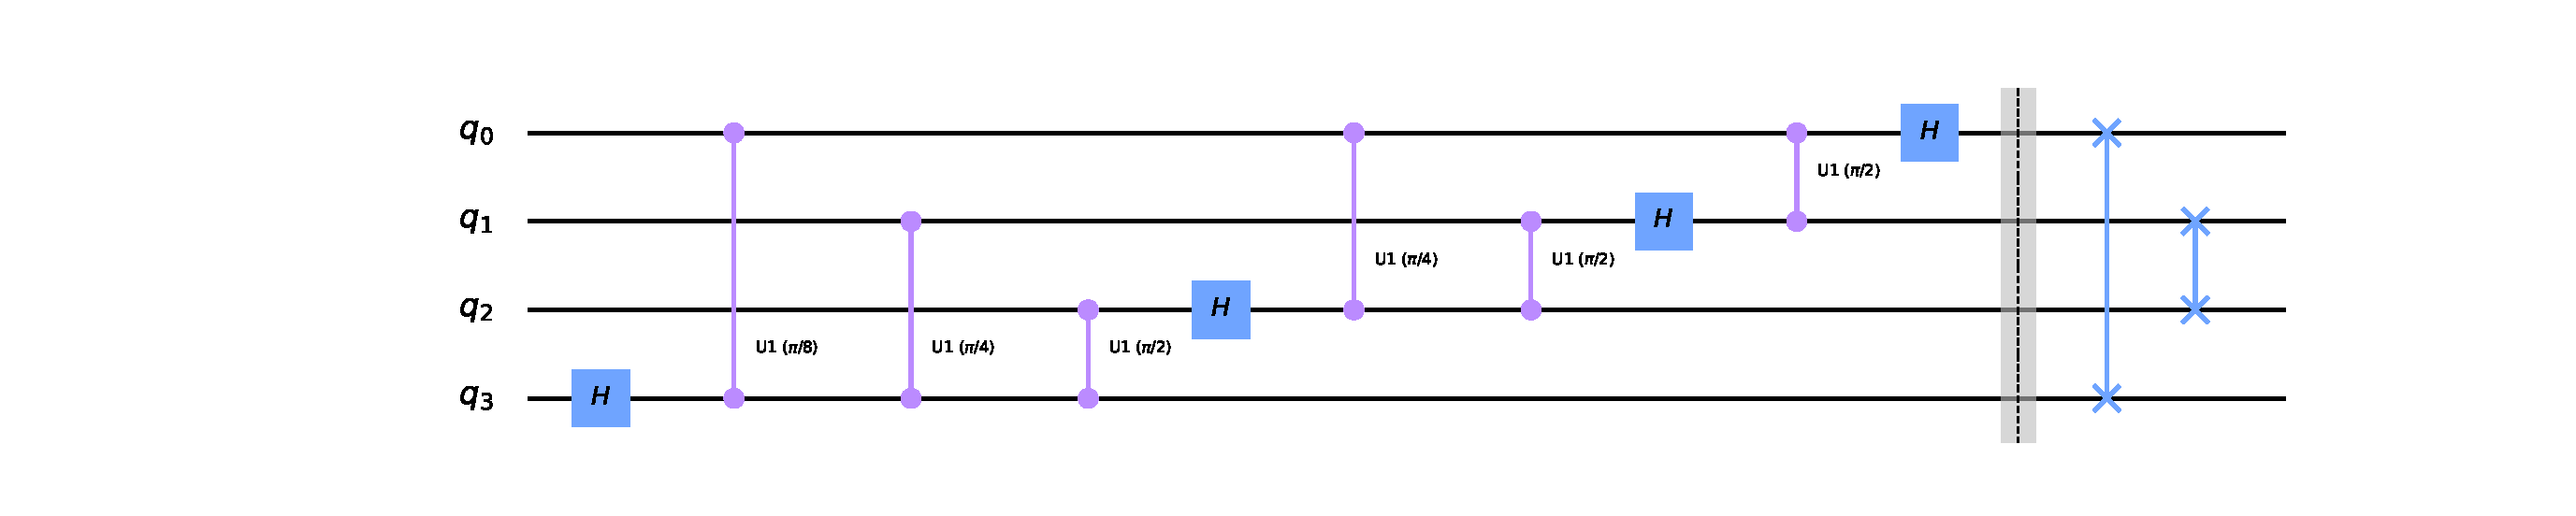
\includegraphics[width=\textwidth]{res/qft-4-qubits-circuit.pdf}
    \caption{Qiskit 4-qubit QFT circuit graph}
    \label{fig:qft-4-qubit-circuit}
\end{figure}

To get the inverse of that circuit \emph{Qiskit} offers the method \texttt{inverse()} which can be applied on any \texttt{QuantumCircuit}.
It is applied in the function displayed in appendix~\ref{subsec:inverse-qft-function} and delivers together with the non-inversed QFT the circuit depicted in figure~\ref{fig:qft-4-qubit-circuit-with-inverse}.

\begin{figure}[H]
    \centering
    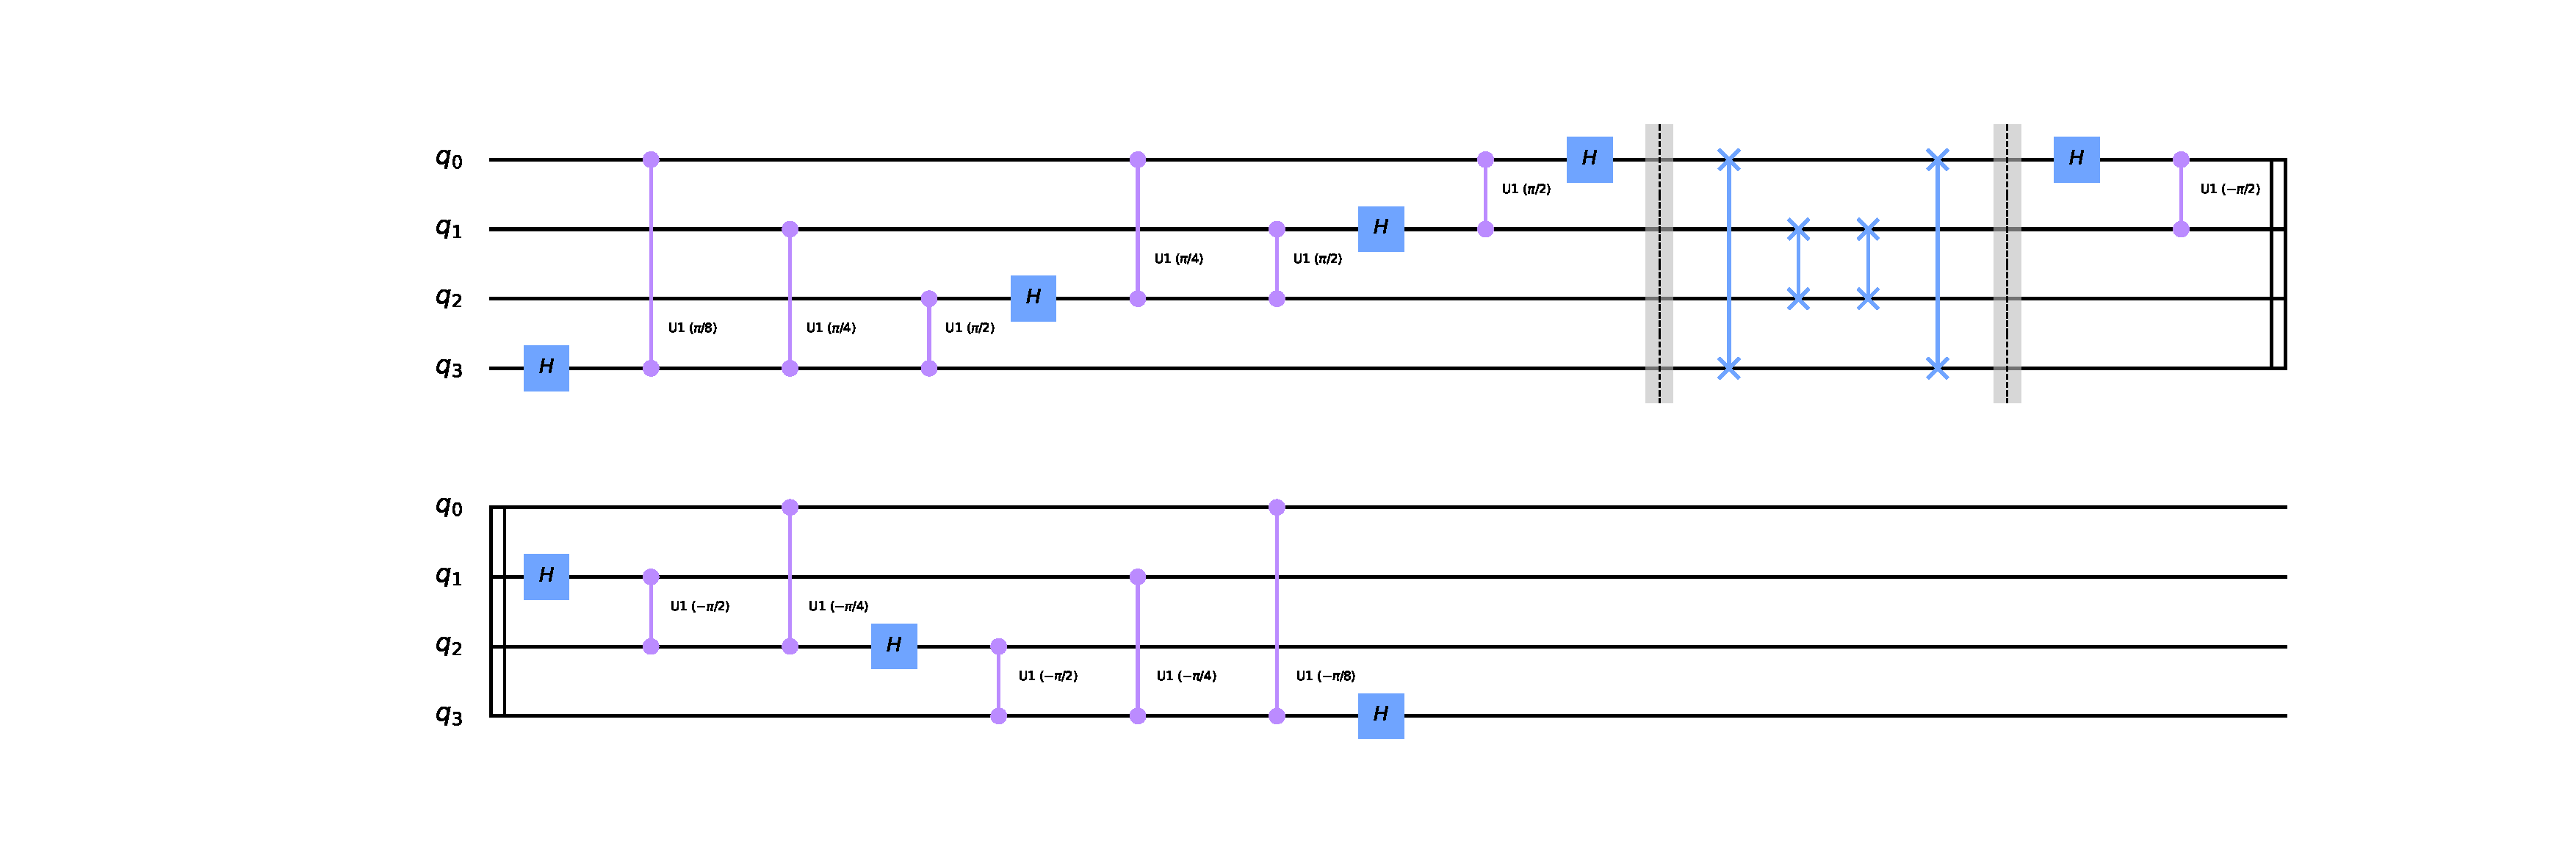
\includegraphics[width=\textwidth]{res/qft-4-qubits-circuit-with-inverse.pdf}
    \caption{Qiskit 4-qubit QFT + inverse QFT circuit}
    \label{fig:qft-4-qubit-circuit-with-inverse}
\end{figure}

The last step to have a fully functional circuit, is to encode a number to the qubits that serve as the input.
A method in appendix~\ref{subsec:encoding-decoding-number-in-circuit} is written that encodes a number to a binary string and later to another quantum circuit that is scaled to fit the amount of needed bits to represent the passed number.
For example the decimal integer number 12 is encoded to the binary string \texttt{1100} and therefore needs the circuit to have 4 input qubits.
Additionally, the same code in the appendix shows a function to measure the qubits to classical bits at the end of the circuit to get the circuits result as binary string again.
That result should ideally match the input when no error occurs.

The full circuit for the encoded number \(6\) (\texttt{110}) is shown in figure~\ref{fig:full-qft-3-qubit-circuit}.

\begin{figure}[H]
    \centering
    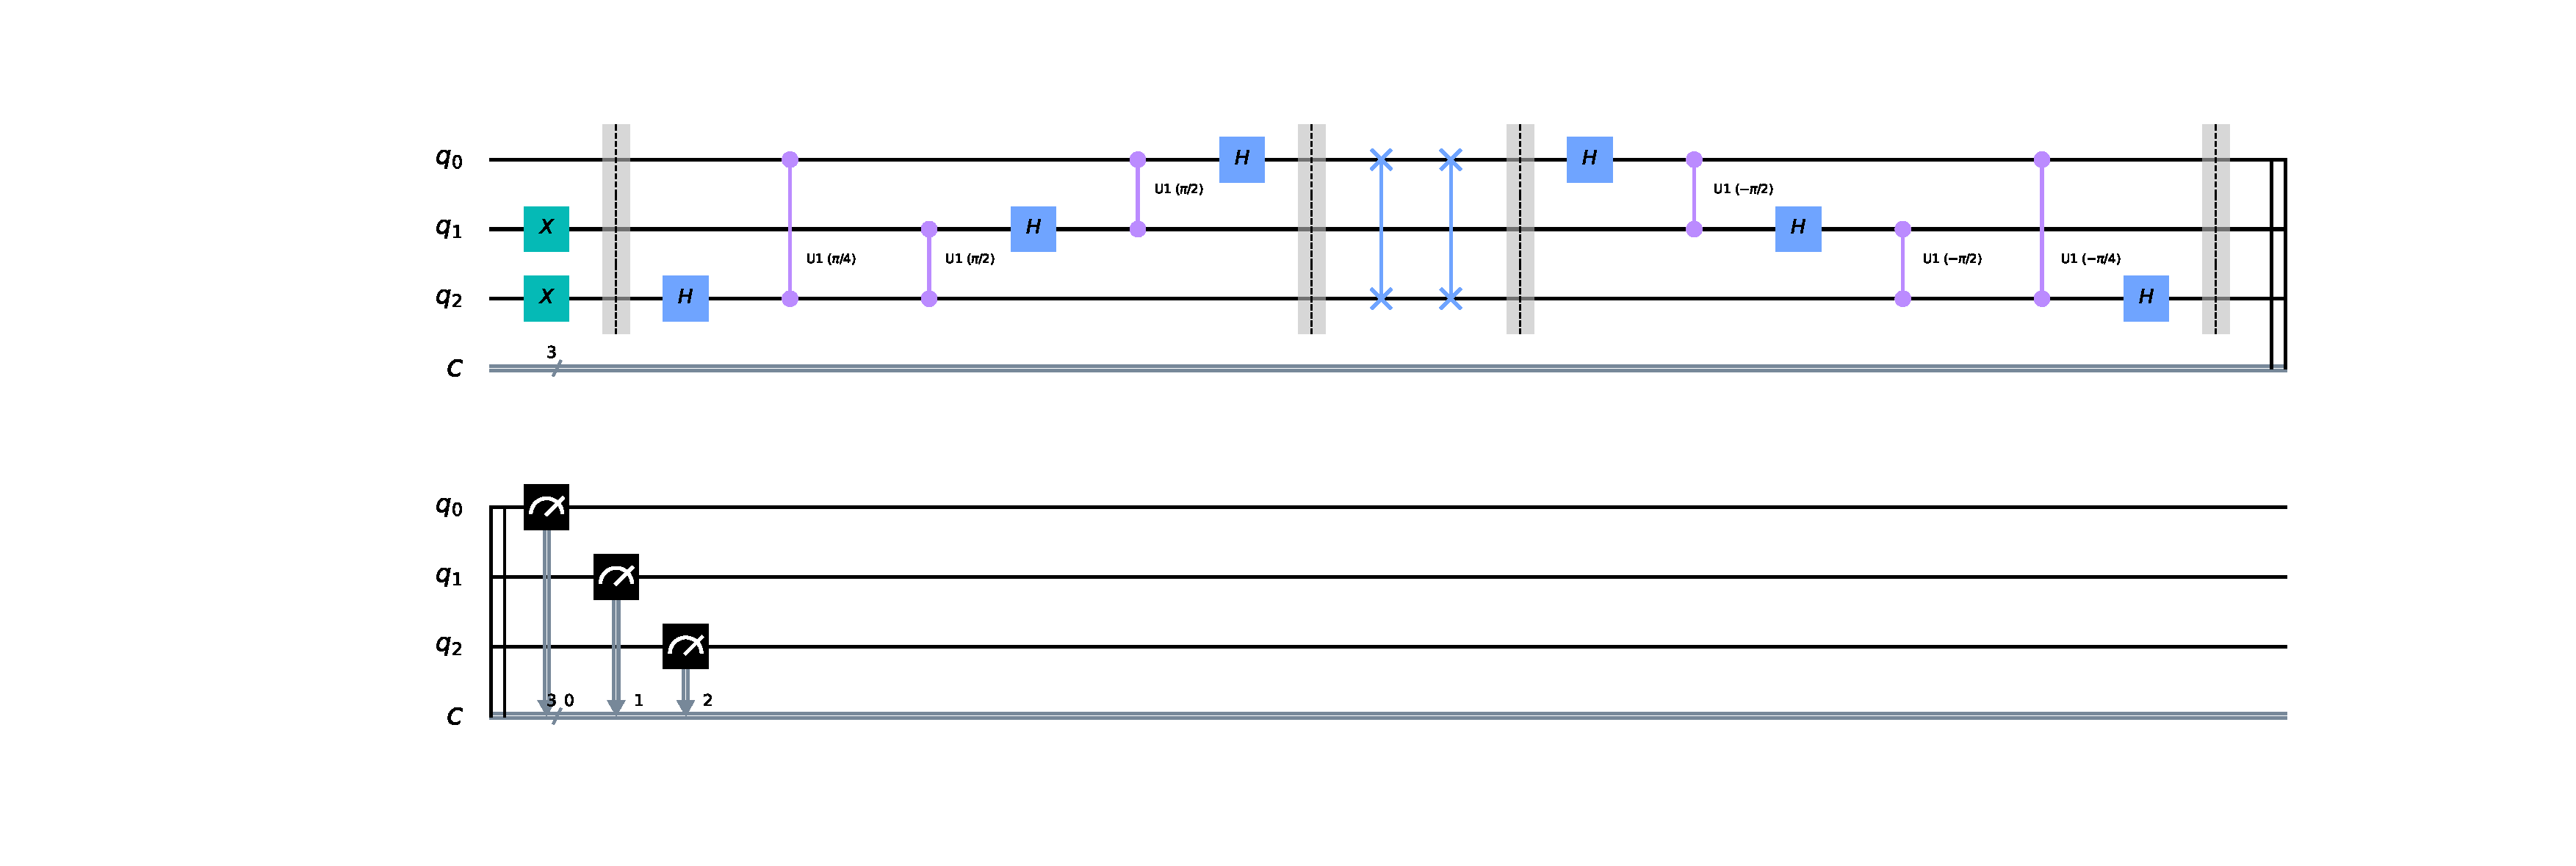
\includegraphics[width=\textwidth]{res/full-qft-3-qubit-circuit.pdf}
    \caption{Qiskit 3-qubit circuit used in this paper}
    \label{fig:full-qft-3-qubit-circuit}
\end{figure}

For the sake of completeness, the source code for generating the above image is listed in Annex~\ref{subsec:generating-full-qft-circuit}.

\paragraph{Testing}

Now that we have the circuit we should be able to test it using the Qiskit simulator and a real quantum device.
The simulator testing is done using the code from~\ref{subsec:testing-circuit-simulator-no-noise} from which figure~\ref{fig:test-histogram} is created.
The histogram is showing \(1024\) simulated results from the circuit.
Since we have not configured the simulator to simulate noise the result is the same (\texttt{110}) for all shots as expected.

\begin{figure}[H]
    \centering
    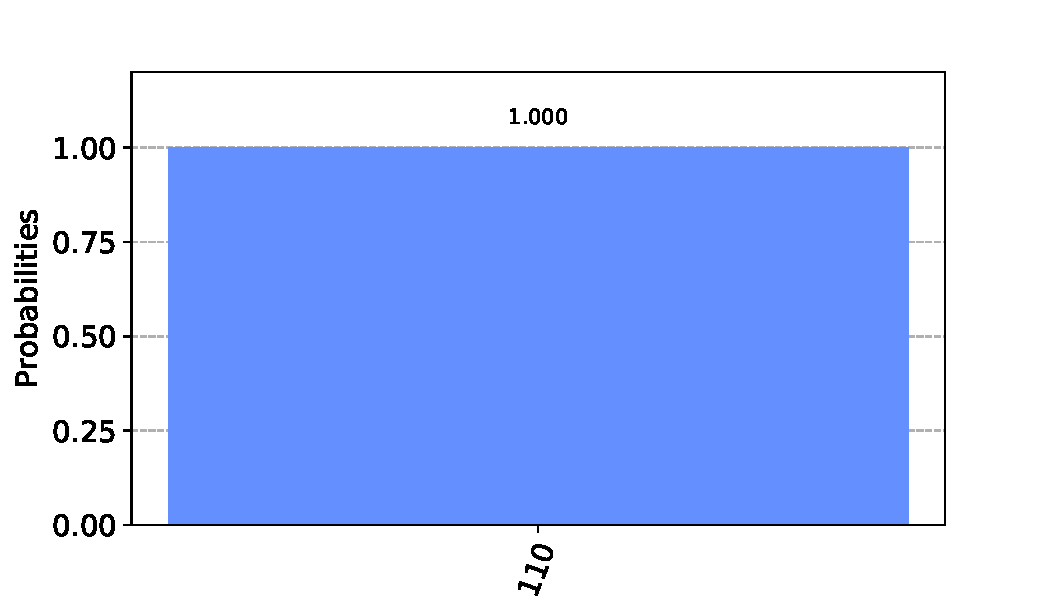
\includegraphics[width=0.7\textwidth]{res/test-histogram.pdf}
    \caption{Simulator result without noise for the full proposed QFT circuit with 3 qubits}
    \label{fig:test-histogram}
\end{figure}

We are able to simulate noise using the \texttt{noise\_model} parameter of Qiskits \texttt{execute} function.
\citeA{QiskitErrorCorrection} showed a function to create a noise model from which we derived the one listed in appendix~\ref{subsec:noise-model-function}.
It anticipated two parameters:
\begin{enumerate}
    \item The probability \(p_{error_{measurement}}\) that the measurement leads to a bit-flip
    \item The probability \(p_{error_{gate}}\) to replace the state of a qubit with a random state
\end{enumerate}

Another way of creating a noise model is by automatically generating one from the properties of a real quantum device using the \texttt{NoiseModel.from\_backend()} method~\cite{QiskitDocsNoise}.
In the first test we'll settle with manually specifying the probabilities to both \(5 \%\).
Later a noise model is generated from a real quantum backend followed by executing the circuit on the real device.

The code for generating the simulated results as shown in the histogram in figure~\ref{fig:test-histogram-with-noise} is listed in appendix~\ref{subsec:testing-circuit-simulator-noise}.
It is evident that there is indeed noise as we do no more measure the correct result \texttt{110} with \(100 \%\) probability.

\begin{figure}[H]
    \centering
    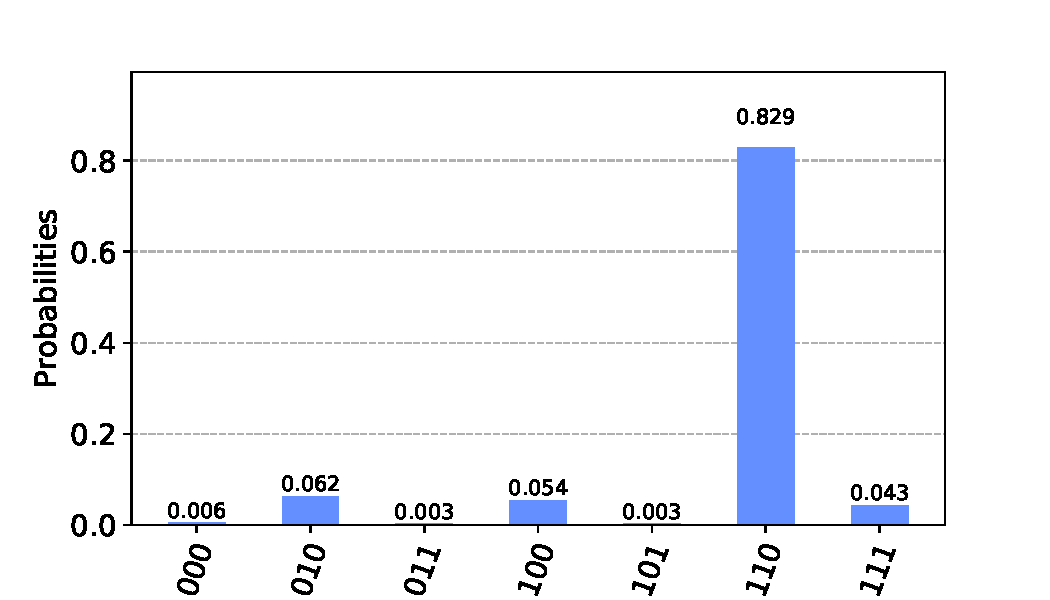
\includegraphics[width=0.7\textwidth]{res/test-histogram-with-noise.pdf}
    \caption{Simulator result \textbf{with} noise for the full proposed QFT circuit with 3 qubits}
    \label{fig:test-histogram-with-noise}
\end{figure}

Now we try generating a noise model from a real quantum backend.
The code to do that is as always placed in the appendix~\ref{subsec:testing-circuit-generated-noise-model}.
It is choosing the least busy quantum device.
In the case of the resulting figure~\ref{fig:test-histogram-generated-noise-model} it has chosen a backend called \texttt{ibmqx2}.
If we compare it with the previous histogram, we find that it has produced a noise model that is not as noisy as the \(5 \%\) gate and measurement errors we selected earlier.

\begin{figure}[H]
    \centering
    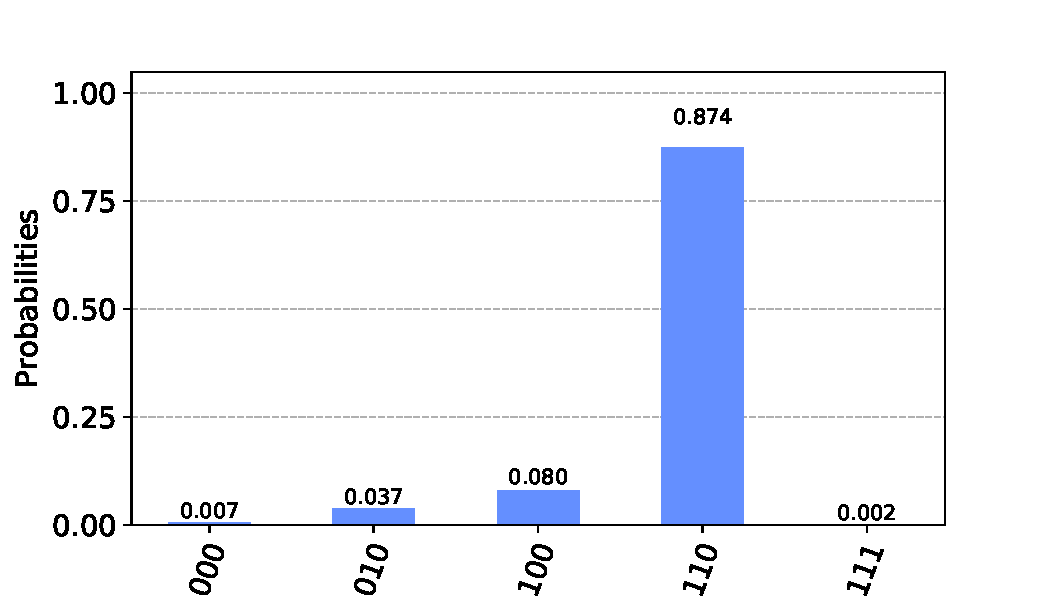
\includegraphics[width=0.7\textwidth]{res/test-histogram-generated-noise-model.pdf}
    \caption{Real quantum device result for the full proposed QFT circuit with 3 qubits}
    \label{fig:test-histogram-generated-noise-model}
\end{figure}

The resulting histogram for the test with a real quantum device, which can be generated using the code from appendix~\ref{subsec:testing-circuit-real-device}, is depicted in figure~\ref{fig:test-histogram-real-device}.
Another result the code is outputting is the quantum backend name on which the circuit has been executed.
In this case the name is \texttt{ibmqx2}.
That happens to be the same that Qiskit has generated a noise model for.
Comparing it to the actual results we see a huge difference as the actual noise seems to be greater.

\begin{figure}[H]
    \centering
    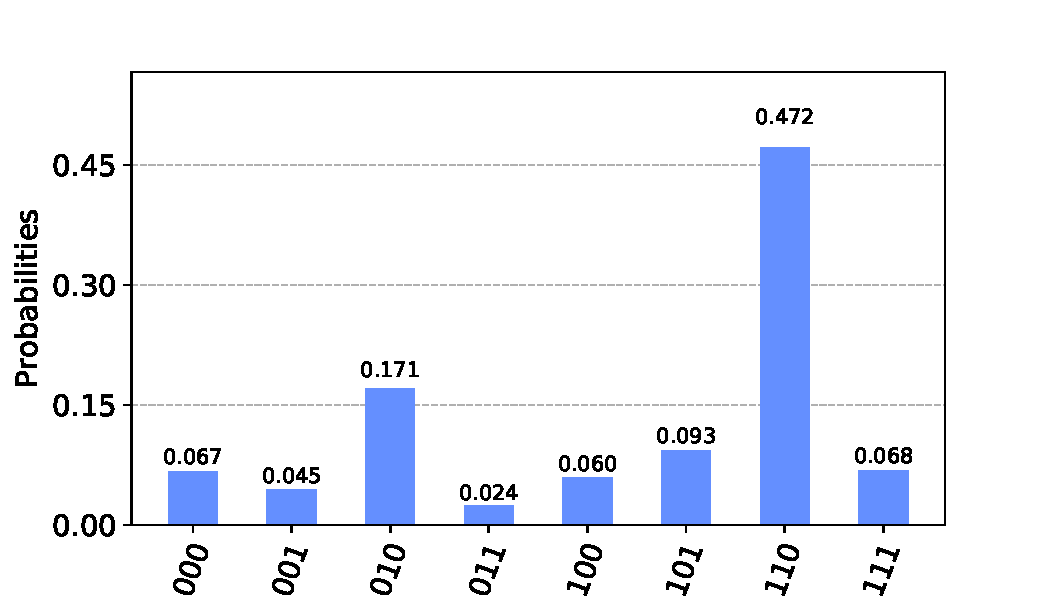
\includegraphics[width=0.7\textwidth]{res/test-histogram-real-quantum-device.pdf}
    \caption{Real quantum device result for the full proposed QFT circuit with 3 qubits}
    \label{fig:test-histogram-real-device}
\end{figure}

\subsection{QFT circuit changes for error-correction}
\label{subsec:qft-circuit-error-correction}

We now are applying some changes in order to correct bit-flip errors in the circuit.
A good result would be a better looking histogram than the ones listed above.

To keep the circuit relatively small we will stick with the 3-qubit QFT circuit and repeat it 3 times.
That means we have to stack the previously shown circuit vertically and add some ancillary qubits.
The functions in appendix~\ref{subsec:modified-qft-circuit-functions} are rewritten versions of the previously shown ones that allow passing a parameter specifying a quantum circuit object to apply the gates on as well a vertical \texttt{offset} to apply them in the passed circuit.
This is done to have the code reusable, small and still comprehensible.

Additionally those functions are used in another function \texttt{prepare\_rc\_qec\_qft\_circuit} which can be seen in appendix~\ref{subsec:circuit-building-code}.
It is building the whole circuit for a specified input number and repetition count.

The last code snipped can be looked up in appendix~\ref{subsec:appendix-decoding-result-circuit} and is decoding a resulting bit string from the circuit.
That means correcting the error when the ancillary bits indicate one.

\paragraph{Testing}

    \section{Summary}
\label{sec:summary}

After having observed some interesting results we want to quickly sum up the contents of the paper followed by some proposals for further studies.

\subsection{Conclusion}
\label{subsec:conclusion}

We have been implementing a quantum circuit trying to error correct bit-flips over several repeated QFT circuits using the Framework Qiskit.
While the Qiskit simulator showed good results for manual as well as automatically configured noise models, current IBMQ backends seem to be still too noisy for the proposed circuit.
Additionally, we are able to say that the generated noise model from Qiskit is not estimating properly - at least for the proposed circuit.

\citeA[p. 1]{tannu2018case} state that we are currently dealing with \emph{Noisy Intermediate Scale Quantum computers} that do not have the capacity to utilize QEC due to the limited amount of qubits available.
That said we could experience a little improvement with the "Paris" backend although we were only correcting bit-flip errors.
They are correct as having proper QEC codes requires a tremendous bigger amount of qubits than we have available today.

Additionally, \citeA[p. 3]{tannu2018case} write that the overall error rate is usually dominated by the gate errors from which we have a lot in the proposed circuit.
Especially the \texttt{CNOT} gate seems to have high error rates which we utilize extensively in the circuit to "read" the current qubit state to the ancillary qubits~\cite[p. 3]{tannu2018case}.
That might be another factor that leads to the observed strong noisy results.

\subsection{Proposals for further studies}
\label{subsec:proposals-for-further-studies}

In summary we find several proposals that might be worth studying in the future:

\begin{itemize}
    \item Since we rely on \texttt{CNOT} gates it would be interesting to remove them from the circuit and afterwards observe what happens to the "Only merged results" histogram.
    \item Qiskit allows us to directly select and assign specific qubits of a real quantum backend that we want to use.
    That way we might be able to use only qubits that have low error rates.
\end{itemize}


    \newpage

    \bibliography{refs}

    \newpage

    \section*{Appendix}
    \label{sec:appendix}

    \subsection*{Test}

\end{document} 
